\pagenumbering{arabic}
\section{需求分析}

\subsection{功能性需求}

整体的系统需求如图2.1所示

\begin{figure}[thbp!]
	\centering
	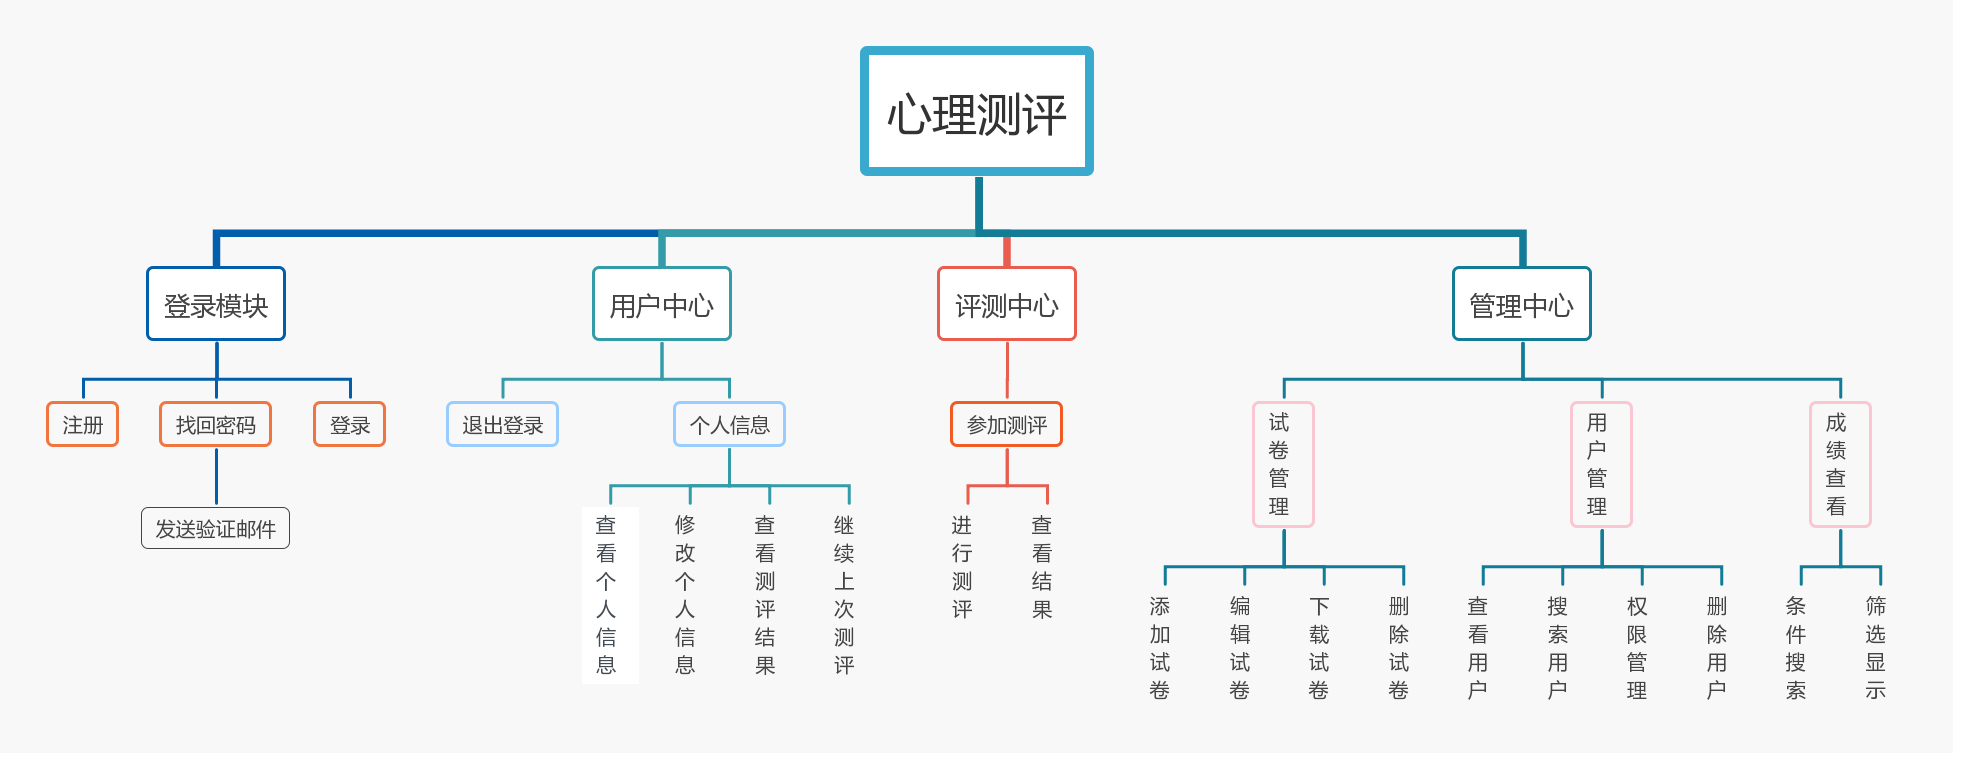
\includegraphics[width=1.0\linewidth]{figure/functions}
	\label{fig:functions} \\
	图2.1 系统总体需求
\end{figure}


整个系统分为四大模块:

(1) 登陆模块:用户可以进行注册、登陆、邮箱激活、找回密码。

(2) 用户中心:用户查看个人信息、查看自己所做试卷和未完成试卷、退出登陆。

(3) 评测中心: 用户进行评测和查看评测结果。

(4) 管理模块:管理员对试卷进行上传、下载、编辑和删除,对用户进行添加、授权和删除,根据成绩筛选用户。

系统的用例图如图2.2所示

\begin{figure}[htp]
	\centering
	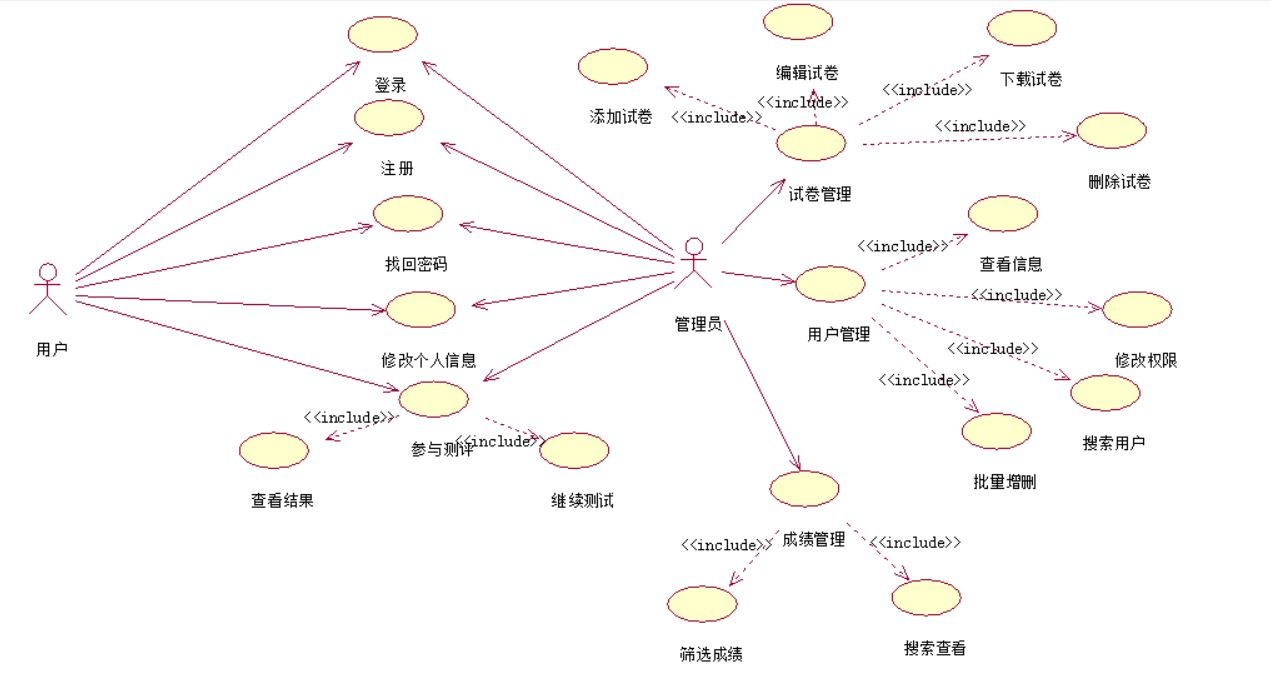
\includegraphics[width=0.7\linewidth]{figure/user_case}
	\label{fig:user_case} \\
	图2.2 系统用例图
\end{figure}

系统分为两种用户:

(1) 普通用户:普通用户可以注册、登陆、找回密码、评测、查看评测信息。

(2) 管理员:管理员有普通用户的所有权限,同时可以管理试卷、用户、成绩。

\subsection{非功能性需求}

(1) 页面响应迅速,不会出现白屏等情况。

(2) 对于难以表述的题目,可选择使用图片、音频等方式进行辅助。

(3) 保护用户隐私,避免个人隐私信息的泄露。

(4) 用户可在疲倦时暂停答题,系统将对已答部分进行保存,下次进入时可选择继续完成。

(5) 整体设计友好温和,尽量不给受测者压力,保障测评结果尽量少受外界因素的干扰。

\subsection{系统目标}

目前网络上较为流行的各类网页式心理测试又存在不系统不完整、信息无法储存、无法管理、无法对比查看、试卷来源不可靠、风险性较高、测试结果不详细没有指导意义等问题。该类测试随机性较大,传播速度快,传播范围广,但是受测者经过一次测试后很难重复测试持续跟踪,也就是说测试结果很难真正的给予受测者实质性的评判依据和进一步的指导,仅仅是停留在非常表面的随手答题阶段。

基于以上客观现实和待解决问题,本次毕设希望做到,每个人可以根据我们系统的分析结果了解当前自己的心理状态,明确自己的目标,改进自己的不足,使得心理测评系统真正的产生实质性功效。